\documentclass[11pt]{article}

\usepackage[margin=1in]{geometry}
\usepackage{amsmath,amssymb}
\usepackage{xcolor}
\usepackage{graphicx}
\usepackage{hyperref}
\usepackage{booktabs}
\usepackage{float}
\usepackage{url}
\usepackage{listings}
\usepackage{tikz}
\usetikzlibrary{arrows.meta,positioning,calc}

\definecolor{codegreen}{rgb}{0,0.6,0}
\definecolor{codegray}{rgb}{0.5,0.5,0.5}
\definecolor{codepurple}{rgb}{0.58,0,0.82}
\definecolor{backcolour}{rgb}{0.95,0.95,0.92}
\definecolor{accent}{HTML}{2E75B6}

\lstdefinestyle{mystyle}{
  backgroundcolor=\color{backcolour},
  commentstyle=\color{codegreen},
  keywordstyle=\color{magenta},
  numberstyle=\tiny\color{codegray},
  stringstyle=\color{codepurple},
  basicstyle=\ttfamily\footnotesize,
  breakatwhitespace=false,
  breaklines=true,
  captionpos=b,
  keepspaces=true,
  numbers=left,
  numbersep=5pt,
  showspaces=false,
  showstringspaces=false,
  showtabs=false,
  tabsize=2
}
\lstset{style=mystyle}

\title{Training Metrics Reference\\
\large What Every Logged Number Means}
\author{Pulak Mehrotra}
\date{April 2026}

\begin{document}
\maketitle
\tableofcontents

All metrics are logged to TensorBoard under \texttt{output/logs/<run-id>/}.
View with \texttt{tensorboard --logdir output/logs/}.
Note: W\&B was disabled (\texttt{--wandb} not passed) for runs~5--7; all plots
are TensorBoard only. To enable W\&B for future runs add \texttt{--wandb} to
the training command.

% ─────────────────────────────────────────────────────────────────────────────
\section{Primary Metric: Pooling Savings}

\textbf{\texttt{eval/pooling\_savings\_mean}} is the number that matters.
It is computed as:
\begin{align}
  \text{pooling\_savings} &= 1 - \text{pooling\_ratio} \\
  \text{pooling\_ratio}   &= \frac{\max_j c_j \cdot N_{\text{MPD}}}{D_{\text{pod}}}
\end{align}
where $c_j$ is the peak load on MPD~$j$, $N_{\text{MPD}}$ is the number of MPDs
in the pod, and $D_{\text{pod}}$ is the total DRAM of the pod.

Intuitively, the pooling ratio measures how much of the shared MPD capacity the
agent wastes by concentrating load.  A ratio of 1.0 means no savings over a
non-pooled baseline; a ratio of 0.8 means 20\% savings.

\begin{itemize}
  \item \textbf{savings $> 0$}: agent improves on baseline.
        Run~5 peaked at $\approx 0.013$--$0.020$.
  \item \textbf{savings $= 0$}: equivalent to no pooling.
  \item \textbf{savings $< 0$}: agent is actively harmful---worse than not pooling.
        Run~6 hit $-0.62$ due to a collapsed policy.
\end{itemize}

\texttt{env/pooling\_ratio} and \texttt{env/pooling\_savings} are the
training-environment versions computed from a single episode mid-training---much
noisier.  \texttt{eval/pooling\_savings\_mean} is cleaner: 10~random pod
mappings on the held-out eval trace.

% ─────────────────────────────────────────────────────────────────────────────
\section{Reward Signals}

\subsection*{\texttt{eval/mean\_reward}}
Mean episode reward on the eval trace (from SB3's \texttt{EvalCallback}).
This is the raw reward sum, not pooling savings.
These two variants are \emph{not} comparable in magnitude ---
run~6's $-244$ vs.\ run~7's $-25$ does \textbf{not} mean run~7 is 10$\times$ better.

% ─────────────────────────────────────────────────────────────────────────────
\subsection*{Shared notation}

Throughout this section, let:
\begin{itemize}
  \item $t$ --- current tick (5-minute resolution); VM $v$ arrives at tick $t$
  \item $i$ --- host receiving the arriving VM
  \item $\mathcal{N}(i)$ --- set of MPDs reachable by host $i$ (from the CXL topology)
  \item $c_j$ --- current load on MPD $j$ (GB), before this allocation
  \item $c_j^{\text{post}}$ --- load on MPD $j$ after this allocation is applied
  \item $D_{\text{pod}}$ --- total DRAM of the pod (GB); used as a normaliser
  \item $\bar{c} = D_{\text{pod}} / N_{\text{MPD}}$ --- fair-share load per MPD (GB)
  \item $\lambda$ --- penalty weight for secondary terms (\texttt{variance\_lambda} or \texttt{reward\_lambda})
\end{itemize}

% ─────────────────────────────────────────────────────────────────────────────
\subsection*{Departure relief $D_j(t,\,W)$}

Variants A and B share a time-weighted departure-relief signal $D_j(t, W)$
that approximates how much load on MPD $j$ will drain within the next $W$ ticks
(default $W = 200$ ticks $\approx$ 16.7 hours).
\begin{equation}
  D_j(t,\,W)
  \;=\;
  \sum_{\substack{v \in \text{active}(j) \\ \text{end}(v) \leq t + W}}
  \!\!
  \text{mem}(v)
  \cdot
  \left(1 - \frac{\text{end}(v) - t}{W}\right)
  \label{eq:Dj}
\end{equation}
where $\text{active}(j)$ is the set of VMs currently allocated on MPD $j$,
and $\text{mem}(v)$ is the GB allocated to VM $v$ on MPD $j$.

The weight $\bigl(1 - (\text{end}(v)-t)/W\bigr)$ is largest for VMs departing
soon and falls to zero for VMs departing exactly at $t+W$.
VMs departing after $t + W$ contribute nothing.

\medskip
\noindent\textbf{Intuition.}
A VM departing in 10 minutes counts almost fully toward relief;
a VM with three days remaining is treated as sticky load and contributes zero.
Two MPDs at identical current load $c_j$ can therefore have very different
projected loads after subtracting $D_j$.

\medskip
\noindent\textbf{Projected sticky load.}
Define the normalised projected load on MPD $j$ after the current allocation:
\begin{equation}
  \hat{c}_j^+(t)
  \;=\;
  \frac{c_j^{\text{post}} - D_j(t,\,W)}{D_{\text{pod}}}
  \label{eq:chat_plus}
\end{equation}
This is the fraction of $D_{\text{pod}}$ that MPD $j$ will still be carrying
once near-term departures drain.  A high $\hat{c}_j^+$ means the MPD will
remain a bottleneck; a low value means load will drain soon.

% ─────────────────────────────────────────────────────────────────────────────
\subsection*{Reward variant A (runs 5, 7)}

Variant A penalises the worst \emph{projected sticky load} among the MPDs
this host can directly reach:
\begin{equation}
  r_t^A
  \;=\;
  -\max_{j \in \mathcal{N}(i)}\,\hat{c}_j^+(t)
  \label{eq:reward_A}
\end{equation}

Every reachable MPD contributes signal at every step, not just the pod-wide
worst.  This makes the reward dense: bad placements onto any reachable MPD
cause an immediate penalty.  Typical episode sum: $-30$ to $-20$.

\medskip
\noindent\textbf{Why this is better than the ``current'' variant.}
$r_t^A$ scores allocations against durable load ($c_j^{\text{post}} - D_j$)
rather than the raw post-allocation peak.  A placement onto a full-but-draining
MPD is penalised less than a placement onto a full-and-sticky MPD, because
$D_j$ subtracts the relief that is already coming.

% ─────────────────────────────────────────────────────────────────────────────
\subsection*{Reward variant B}

Variant B extends A with a penalty for hot MPDs that the current host
\emph{cannot} reach.  Those MPDs are shared with neighboring hosts, so
overloading them harms future placements that those neighbors will attempt.

Let $\bar{\mathcal{N}}(i) = \{1,\ldots,N_{\text{MPD}}\} \setminus \mathcal{N}(i)$
be the set of MPDs unreachable by host $i$.  Define the normalised pre-allocation
projected load on an unreachable MPD:
\begin{equation}
  P_j(t)
  \;=\;
  \frac{c_j - D_j(t,\,W)}{D_{\text{pod}}},
  \quad j \notin \mathcal{N}(i)
  \label{eq:Pj}
\end{equation}
Note that $c_j$ here is the \emph{pre}-allocation load (unreachable MPDs are
unchanged by this step).  Then:
\begin{equation}
  r_t^B
  \;=\;
  r_t^A
  \;-\;
  \lambda \cdot \max_{j \in \bar{\mathcal{N}}(i)} P_j(t)
  \label{eq:reward_B}
\end{equation}
with $\lambda = 0.2$ by default (\texttt{reward\_lambda}).

The global term discourages a host from saturating shared MPDs even when its
own reachable set looks comfortable, capturing indirect congestion effects that
$r_t^A$ alone cannot see.

% ─────────────────────────────────────────────────────────────────────────────
\subsection*{Reward variant ``current'' (run 6)}

The original reward penalises the \emph{increase in raw peak} normalized by
fair share, plus a variance penalty over all MPD loads:
\begin{align}
  r_t^{\text{cur}}
  &= -\frac{c_{\max}^{\text{post}} - c_{\max}}{\bar{c}}
     \;-\;
     \lambda \cdot \mathrm{Var}\!\left(\frac{c_j}{\bar{c}}\right)
  \label{eq:reward_cur}
  \\[4pt]
  \text{where}\quad
  c_{\max} &= \max_j c_j,
  \quad
  c_{\max}^{\text{post}} = \max_j c_j^{\text{post}},
  \quad
  \bar{c} = \frac{D_{\text{pod}}}{N_{\text{MPD}}}
  \notag
\end{align}
with $\lambda = 0.5$ (\texttt{variance\_lambda}).

\medskip
\noindent\textbf{Why this variant failed (run 6).}
\begin{itemize}
  \item \textbf{Single-MPD signal.}
        $c_{\max}^{\text{post}} - c_{\max}$ is nonzero only when the
        allocation lands on the \emph{current} worst MPD or creates a new
        worst MPD.  All other placements return $r = -\lambda \cdot \mathrm{Var}(\cdot)$,
        which is the same regardless of which MPD is chosen ---
        giving the policy almost no gradient for distinguishing good from bad placements
        on non-worst MPDs.
  \item \textbf{No departure model.}
        $c_j$ treats a VM departing in 10 minutes identically to one with
        3 days remaining.  The policy has no signal to prefer draining MPDs.
  \item \textbf{Result.}
        SAC collapsed all allocations onto one or two MPDs;
        max/min load ratio $\sim 20\times$; greedy outperformed the learned policy.
\end{itemize}

% ─────────────────────────────────────────────────────────────────────────────
\subsection*{Comparison}

\begin{center}
\small
\renewcommand{\arraystretch}{1.3}
\begin{tabular}{p{0.16\linewidth}p{0.22\linewidth}p{0.22\linewidth}p{0.30\linewidth}}
\toprule
\textbf{Variant} & \textbf{Signal scope} & \textbf{Departure-aware} & \textbf{Key failure mode} \\
\midrule
\texttt{current} & Single worst MPD & No & Degenerate: all load collapses to one MPD \\
A                & All reachable MPDs & Yes ($D_j$) & Blind to shared-MPD congestion \\
B                & All MPDs (local + global) & Yes ($D_j$) & None identified yet; ablation pending \\
\bottomrule
\end{tabular}
\end{center}

\subsection*{\texttt{eval/mean\_ep\_length}}
Average episode length in VM arrival events.  Typical: 6{,}000--8{,}000.
Very low values suggest trace loading or HOTFIX filter issues.

% ─────────────────────────────────────────────────────────────────────────────
\section{SAC Internals}

% ─────────────────────────────────────────────────────────────────────────────
\subsection*{What SAC is doing}

Soft Actor--Critic (SAC) \cite{haarnoja2018sac} maximises a reward objective
augmented with a policy-entropy bonus:
\begin{equation}
  J(\pi)
  = \mathbb{E}_{\tau \sim \pi}
    \!\left[\,
      \sum_{t=0}^{T} \gamma^t
      \Bigl(r_t + \alpha\,\mathcal{H}\!\left(\pi(\cdot \mid s_t)\right)\Bigr)
    \right]
  \label{eq:sac_obj}
\end{equation}
where $\mathcal{H}(\pi(\cdot|s)) = -\mathbb{E}_{a \sim \pi}[\log \pi(a|s)]$
is the Shannon entropy of the policy at state $s$,
$\alpha > 0$ is the \emph{entropy coefficient} (temperature),
and $\gamma = 0.999$ in this project.

The entropy term keeps the policy stochastic: it is rewarded for spreading
probability mass across good actions rather than collapsing to a single deterministic
choice.  Without it, the policy converges prematurely to a local optimum.

\medskip

Figure~\ref{fig:sac_arch} shows the components.  All five interact at every
gradient update.

\begin{figure}[H]
\centering
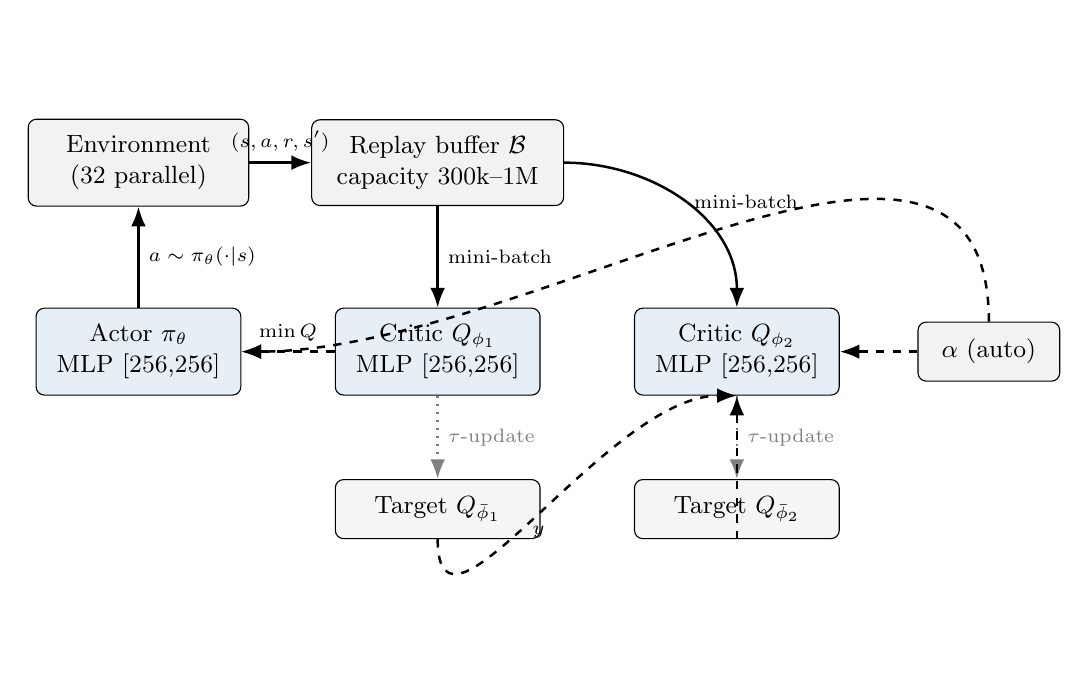
\begin{tikzpicture}[
    every node/.style={font=\small},
    box/.style={draw, rounded corners=3pt, fill=black!5,
                minimum height=0.75cm, align=center, inner sep=6pt},
    netbox/.style={draw, rounded corners=3pt, fill=accent!12,
                   minimum height=0.75cm, align=center, inner sep=6pt},
    arr/.style={-{Latex[length=2.5mm]}, line width=0.9pt},
    darr/.style={-{Latex[length=2.5mm]}, line width=0.9pt, dashed},
    polyak/.style={-{Latex[length=2.5mm]}, line width=0.9pt, dotted, gray}
]

% ── Replay buffer ─────────────────────────────────────────────────────────
\node[box, minimum width=3.2cm] (buf) at (0, 0) {Replay buffer $\mathcal{B}$\\capacity 300k--1M};

% ── Environment ───────────────────────────────────────────────────────────
\node[box, minimum width=2.8cm] (env) at (-3.8, 0) {Environment\\(32 parallel)};
\draw[arr] (env) -- node[above, font=\scriptsize]{$(s,a,r,s')$} (buf);

% ── Actor ─────────────────────────────────────────────────────────────────
\node[netbox, minimum width=2.6cm] (actor) at (-3.8, -2.4)
      {Actor $\pi_\theta$\\MLP [256,256]};
\draw[arr] (actor) -- node[right, font=\scriptsize]{$a \sim \pi_\theta(\cdot|s)$} (env);

% ── Critic 1 ──────────────────────────────────────────────────────────────
\node[netbox, minimum width=2.6cm] (q1) at (0, -2.4)
      {Critic $Q_{\phi_1}$\\MLP [256,256]};

% ── Critic 2 ──────────────────────────────────────────────────────────────
\node[netbox, minimum width=2.6cm] (q2) at (3.8, -2.4)
      {Critic $Q_{\phi_2}$\\MLP [256,256]};

% ── Target networks ───────────────────────────────────────────────────────
\node[box, minimum width=2.6cm, fill=gray!8] (tq1) at (0, -4.4)
      {Target $Q_{\bar\phi_1}$};
\node[box, minimum width=2.6cm, fill=gray!8] (tq2) at (3.8, -4.4)
      {Target $Q_{\bar\phi_2}$};

% ── Alpha ─────────────────────────────────────────────────────────────────
\node[box, minimum width=1.8cm] (alpha) at (7.0, -2.4)
      {$\alpha$ (auto)};

% ── Replay buffer → critics ───────────────────────────────────────────────
\draw[arr] (buf) -- node[right, font=\scriptsize]{mini-batch} (q1);
\draw[arr] (buf.east) to[out=0,in=90] node[right, font=\scriptsize]{mini-batch} (q2.north);

% ── Critics → actor ───────────────────────────────────────────────────────
\draw[darr] (q1) -- node[above, font=\scriptsize]{$\min Q$} (actor);

% ── Polyak update: critics → targets ─────────────────────────────────────
\draw[polyak] (q1) -- node[right, font=\scriptsize]{$\tau$-update} (tq1);
\draw[polyak] (q2) -- node[right, font=\scriptsize]{$\tau$-update} (tq2);

% ── Targets → Bellman target ──────────────────────────────────────────────
\draw[darr] (tq1.south) to[out=-90,in=180] node[below, font=\scriptsize]{$y$} (q2.south);
\draw[darr] (tq2.south) -- (q2.south);

% ── Alpha → actor + critics ───────────────────────────────────────────────
\draw[darr] (alpha) -- (q2);
\draw[darr] (alpha.north) to[out=90,in=0] (actor.east);

\end{tikzpicture}
\caption{SAC architecture as used in this project.
  Solid arrows: data flow during training (mini-batches from replay buffer).
  Dashed: gradient-coupled terms.
  Dotted: Polyak target-network update ($\tau = 0.005$).
  The two critics independently estimate $Q$; their minimum is used everywhere
  to suppress overestimation.}
\label{fig:sac_arch}
\end{figure}

% ─────────────────────────────────────────────────────────────────────────────
\subsection*{Critic update --- Bellman residual}

SAC maintains two independent critic networks $Q_{\phi_1}$, $Q_{\phi_2}$
(the ``clipped double-Q'' trick from TD3 \cite{fujimoto2018td3}) to suppress
Q-value overestimation.

At each gradient step, a mini-batch
$(s, a, r, s') \sim \mathcal{B}$ is drawn from the replay buffer.
The \emph{Bellman target} is computed using the frozen target networks
$Q_{\bar\phi_1}$, $Q_{\bar\phi_2}$:
\begin{equation}
  y
  = r + \gamma
    \underbrace{
      \left(
        \min_{i=1,2} Q_{\bar\phi_i}(s', \tilde{a}')
        - \alpha \log \pi_\theta(\tilde{a}' \mid s')
      \right)
    }_{\text{soft value of next state } V(s')}
  , \quad
  \tilde{a}' \sim \pi_\theta(\cdot \mid s')
  \label{eq:bellman_target}
\end{equation}

The subtracted $\alpha \log \pi$ term is the entropy bonus: the policy is
credited for being uncertain about the next action.  The $\min$ across the two
target critics suppresses over-optimistic bootstrapping.

Both critics are then updated by minimising mean-squared Bellman error:
\begin{equation}
  \mathcal{L}_{\text{critic}}
  = \mathbb{E}_{(s,a,r,s') \sim \mathcal{B}}
    \!\left[
      \frac{1}{2}\sum_{i=1}^{2}
      \Bigl(Q_{\phi_i}(s,a) - y\Bigr)^2
    \right]
  \label{eq:critic_loss}
\end{equation}

\noindent\textbf{Project values.} $\gamma = 0.999$, \texttt{batch\_size} = 256 (fast: 512),
\texttt{learning\_starts} = 1{,}000 (no updates until buffer has at least 1k transitions).

% ─────────────────────────────────────────────────────────────────────────────
\subsection*{Actor update --- entropy-regularised policy gradient}

The actor is updated to maximise Q-value while also maximising entropy.
Concretely, the actor loss is:
\begin{equation}
  \mathcal{L}_{\text{actor}}
  = \mathbb{E}_{s \sim \mathcal{B},\; \tilde{a} \sim \pi_\theta(\cdot|s)}
    \!\left[
      \alpha \log \pi_\theta(\tilde{a} \mid s)
      - \min_{i=1,2} Q_{\phi_i}(s, \tilde{a})
    \right]
  \label{eq:actor_loss}
\end{equation}

Minimising $\mathcal{L}_{\text{actor}}$ does two things simultaneously:
\begin{itemize}
  \item The $-Q$ term pushes the actor toward actions with high Q-value
        (exploit what the critics have learned).
  \item The $+\alpha \log \pi$ term penalises deterministic policies
        (low-entropy distributions have high $\log \pi$ under the chosen action).
\end{itemize}

Note: the Q-values used here are from the \emph{live} critics $\phi_i$,
not the frozen targets.  Gradients flow through $\pi_\theta$ but not $Q_{\phi_i}$.

\noindent\textbf{What the logged metric means.}
\texttt{sac/actor\_loss} = the value of $\mathcal{L}_{\text{actor}}$ at the last
gradient step.  It becomes more negative as the policy improves
(higher Q-values dominate).  A \emph{rising} or \emph{flat} actor loss with bad
pooling savings usually means the critic has converged to accurately predict the
value of a \emph{bad} policy --- the actor is optimising toward the wrong target.

% ─────────────────────────────────────────────────────────────────────────────
\subsection*{Automatic entropy tuning ($\alpha$)}

SAC automatically tunes $\alpha$ so that the policy maintains a target entropy
$\mathcal{H}_{\text{target}}$.  SB3 defaults this to $-\dim(\mathcal{A})$, the
negative of the action dimension.
The loss for $\alpha$ is:
\begin{equation}
  \mathcal{L}_{\alpha}
  = \mathbb{E}_{s \sim \mathcal{B},\; \tilde{a} \sim \pi_\theta(\cdot|s)}
    \!\left[
      -\alpha
      \bigl(
        \log \pi_\theta(\tilde{a} \mid s) + \mathcal{H}_{\text{target}}
      \bigr)
    \right]
  \label{eq:alpha_loss}
\end{equation}

If the policy's entropy $-\log \pi$ falls \emph{below} $\mathcal{H}_{\text{target}}$,
the gradient increases $\alpha$ (more exploration pressure).
If entropy is already above target, $\alpha$ decreases.
$\alpha$ is stored as $\log\alpha$ internally to keep it positive;
\texttt{sac/ent\_coef} reports $\exp(\log\alpha)$.

\begin{itemize}
  \item \textbf{Healthy}: 0.1--1.0, declining slowly as the policy specialises.
  \item \textbf{Collapsed} ($\alpha < 0.01$): policy became deterministic too early,
        stuck in a local optimum.  Run~6 hit $\alpha = 0.00079$ at 560k steps ---
        the policy was packing all load onto one MPD with near-zero variance in
        its action.
  \item \textbf{Too high} ($\alpha > 2$): too much noise, policy not committing
        to good allocations.
\end{itemize}

% ─────────────────────────────────────────────────────────────────────────────
\subsection*{Target network update (Polyak averaging)}

After every gradient step the target critics $\bar\phi_i$ are moved slightly
toward the live critics:
\begin{equation}
  \bar\phi_i \;\leftarrow\; \tau\,\phi_i + (1-\tau)\,\bar\phi_i
  \label{eq:polyak}
\end{equation}
with $\tau = 0.005$ (\texttt{tau}).  The target networks lag behind the live
critics, preventing the Bellman target $y$ from moving too fast and causing
divergence.  The smaller $\tau$ is, the more stable but slower the bootstrap.

% ─────────────────────────────────────────────────────────────────────────────
\subsection*{Metric-by-metric reference}

\paragraph{\texttt{sac/q1\_mean}, \texttt{sac/q2\_mean}.}
Mean of $Q_{\phi_1}(s,a)$ and $Q_{\phi_2}(s,a)$ sampled from the replay buffer.
Should rise as the policy improves (higher expected discounted return).
If they grow without bound the critics are overestimating --- the $\min$ trick
only suppresses this partially.
The two critics should track each other: large systematic divergence means one
critic is miscalibrated.

\paragraph{\texttt{sac/q\_spread}.}
$\mathbb{E}|Q_{\phi_1}(s,a) - Q_{\phi_2}(s,a)|$ from a sampled mini-batch.
This measures critic disagreement.
Values below~0.1 mean the critics agree; above~0.5 suggests the value landscape
is shifting faster than the critics can track.

\paragraph{\texttt{sac/critic\_loss}.}
$\mathcal{L}_{\text{critic}}$ (Eq.~\ref{eq:critic_loss}) at the last gradient step.
Should decrease over training.
\textbf{Caution:} near-zero critic loss with bad pooling savings means
the critics have accurately learned the value of a \emph{bad} policy ---
not that the policy is good.
This is the most common misleading signal in run~6.

\paragraph{\texttt{sac/actor\_loss}.}
$\mathcal{L}_{\text{actor}}$ (Eq.~\ref{eq:actor_loss}).
Becomes more negative as Q-values rise.
A flat or rising actor loss with stable critic loss is the classic sign that
the actor is stuck at a local optimum the critics have accurately valued.

\paragraph{\texttt{sac/actor\_grad\_norm}, \texttt{sac/critic\_grad\_norm}.}
$\ell_2$ norm of all gradient tensors in the actor and critic networks
respectively, computed as $\|\nabla\|_2 = \sqrt{\sum_p \|\nabla_p\|_2^2}$.
\begin{itemize}
  \item Critic norm rising sharply (e.g.\ 65 in run~7 late stage): large Bellman
        errors, value landscape changing fast; consider reducing \texttt{learning\_rate}.
  \item Any norm $> 100$: potential instability; gradient clipping may help.
  \item Actor grad norm $\to 0$: actor not updating, effectively frozen.
        Check entropy collapse.
\end{itemize}

\paragraph{\texttt{train/n\_updates}.}
Cumulative gradient steps taken.  Each step draws one mini-batch and runs one
pass through Eqs.~\ref{eq:critic_loss}--\ref{eq:alpha_loss}.
The update rate is determined by \texttt{train\_freq} and \texttt{n\_envs}:
\begin{equation}
  \text{updates}
  = \frac{\text{total\_timesteps}}{\texttt{train\_freq} \times \texttt{n\_envs}}
\end{equation}
Run~7 (\texttt{train\_freq}=8, \texttt{n\_envs}=32, 2M steps):
$2{,}000{,}000 / (8 \times 32) = 7{,}812$ updates --- exactly what was logged.
Run~6 (\texttt{train\_freq}=1, \texttt{n\_envs}=8): $\sim$70k updates at 560k
steps, which is why it was 10$\times$ slower per wall-clock minute.

% ─────────────────────────────────────────────────────────────────────────────
\section{Environment Metrics}

\subsection*{\texttt{env/max\_peak}}
Peak MPD load (GB) seen in the last training episode.  Absolute value depends
on the pod's total DRAM.  Useful for checking trace diversity across envs.

\subsection*{\texttt{env/num\_events}}
Number of VM arrival events in the episode.  Varies by pod and trace.
Typical: 5{,}000--10{,}000.

% ─────────────────────────────────────────────────────────────────────────────
\section{Throughput}

\subsection*{\texttt{time/fps}}
Timesteps per second (SB3 ``frames per second''), including env step, policy
inference, and gradient update.

\begin{center}
\begin{tabular}{llll}
\toprule
Run & fps & n\_envs & Cause of deviation \\
\midrule
Run 5 & 244 & 32 & Healthy baseline \\
Run 7 & 52  & 32 & CPU contention (run~6 running in parallel) \\
Run 6 & 22  & 8  & train\_freq=1, gradient updates dominating \\
\bottomrule
\end{tabular}
\end{center}

% ─────────────────────────────────────────────────────────────────────────────
\section{Augmentation Metrics}
Only logged when \texttt{--augmentation} is enabled (runs 5 and 7).

\subsection*{\texttt{aug/scale\_mean}, \texttt{aug/scale\_std}}
Distribution of memory scaling factors applied to episodes.  Should stay
near $[0.7, 1.2]$ with mean $\approx 0.95$.

\subsection*{\texttt{aug/link\_failures\_applied}}
Count of episodes with random topology link failures.  Zero in runs 5/7
(\texttt{aug\_link\_failures=0.0}).

\subsection*{\texttt{aug/unique\_traces}}
Number of distinct traces seen in the last logging window.
With \texttt{multi\_trace=True} and 10 traces, expect $\sim10$ after warmup.

% ─────────────────────────────────────────────────────────────────────────────
\section{Fault Diagnosis Table}

\begin{center}
\begin{tabular}{p{6cm}p{8cm}}
\toprule
Symptom & Likely cause \\
\midrule
\texttt{pooling\_savings} $< 0$ &
  Policy collapsed; always allocates to one MPD. \\
\texttt{ent\_coef} $\to 0$ early &
  Over-updating (\texttt{train\_freq} too low) or poorly tuned entropy target. \\
\texttt{q1\_mean} exploding &
  Q-value overestimation; try lower learning rate or smaller network. \\
\texttt{critic\_loss} $\approx 0$ but bad savings &
  Critic converged to accurately predict a bad policy's values. \\
\texttt{fps} $\ll$ expected &
  CPU contention; too many parallel envs for available cores. \\
\texttt{pooling\_savings\_std} high &
  Policy inconsistent across pod mappings; may need more training or augmentation. \\
Actor grad norm $\to 0$ &
  Actor stuck; policy not improving. \\
Critic grad norm $\gg 50$ &
  Value landscape shifting fast; consider lower learning rate or grad clipping. \\
\bottomrule
\end{tabular}
\end{center}

% ─────────────────────────────────────────────────────────────────────────────
\section{Reward Function Design --- Best Practices}

The results across runs 5--7 show a consistent ceiling of $\sim$1--1.6\% pooling
savings, policy entropy collapse by 100k steps, and no clear improvement from
longer training.  These are all symptoms of a misdesigned reward function.
This section documents best practices from recent ML literature and maps them
directly onto the failure modes observed here.

% ─────────────────────────────────────────────────────────────────────────────
\subsection{Align the reward with the true objective, not a proxy}

The most dangerous mistake in reward design.
Our reward measures $\Delta\text{peak}$ (immediate MPD load change per step),
but the true objective is \emph{episode-level pooling savings}---a quantity
that only manifests at the end of 7{,}000+ steps.
These diverge because:

\begin{itemize}
  \item An agent can minimise $\Delta\text{peak}$ at every step by spreading
        load uniformly, even when this creates future fragmentation that prevents
        large VMs from fitting efficiently.
  \item The $D_j$ lookahead term attempts to compensate by encoding near-future
        departures, but as the \emph{Noisy Future Knowledge} analysis
        (Uzeel, 2025, internal) shows: if each allocation decision is off by even
        5\%, compounded predictions over 8 days do \emph{worse than greedy}.
        This exactly explains the observed savings ceiling.
\end{itemize}

\noindent\textbf{Fix direction.}
Use the episode-level pooling savings as the terminal reward, with
\emph{potential-based shaping} (Section~\ref{sec:pbrs}) as the only source of
dense intermediate signal.  This is theoretically grounded and cannot change
the optimal policy~\cite{ng1999pbrs}.

% ─────────────────────────────────────────────────────────────────────────────
\subsection{Potential-based reward shaping (PBRS)}
\label{sec:pbrs}

Ng, Harada, and Russell (1999)~\cite{ng1999pbrs} proved that an agent's set of
optimal policies is preserved \emph{if and only if} shaping rewards take the form:
\begin{equation}
  F(s, s') = \gamma\,\Phi(s') - \Phi(s)
  \label{eq:pbrs}
\end{equation}
where $\Phi : \mathcal{S} \to \mathbb{R}$ is an arbitrary \emph{potential function}.
Any other dense reward formulation risks making a suboptimal allocation globally
optimal under the shaped objective.

\noindent Our current reward is \emph{not} in this form---$-({\Delta\text{peak}}/{\bar c})$
adds information about the transition that is not expressible as a potential difference,
so it can (and does) induce a different optimal policy than the true objective.

\noindent\textbf{Valid potential for this system.}
A natural choice is the negative normalised peak:
\begin{equation}
  \Phi(s) = -\frac{\max_j c_j}{D_{\text{pod}}}
\end{equation}
Then $F(s,s') = \gamma\Phi(s') - \Phi(s)$ rewards reductions in the peak MPD
load in a policy-invariant way.
Combined with the sparse terminal reward (true pooling savings), this provides
dense learning signal without distorting the objective.
Recent work~\cite{pbrs2025} shows a linear shift of $\Phi$ can improve convergence
speed without changing the encoded preference.

% ─────────────────────────────────────────────────────────────────────────────
\subsection{Do not mix incommensurable objectives with a fixed $\lambda$}

The \texttt{current} reward variant (Eq.~\ref{eq:reward_cur}) mixes two terms:
peak reduction and load variance, with $\lambda = 0.5$ fixed for all of training.
This is problematic on two levels:

\begin{enumerate}
  \item \textbf{The right trade-off changes during training.}
        Early in training, the policy is random and load variance is high; $\lambda$
        should down-weight the variance term.  Later, once peak is controlled,
        variance matters more.  A fixed scalar cannot adapt.

  \item \textbf{The variance term is semantically wrong for this topology.}
        Equal load across MPDs is impossible---some MPDs serve more hosts and will
        always carry more traffic.  Penalising variance rewards the policy for
        replicating a uniform distribution that the topology does not support.
\end{enumerate}

\noindent\textbf{Principled alternatives.}
Multi-reward RL literature~\cite{multireward2024} recommends:
\begin{itemize}
  \item \textbf{Dynamic weight scheduling:} adjust $\lambda$ via a bandit
        algorithm based on which objective is most violated at each stage.
  \item \textbf{Lexicographic reward:} first optimise the primary objective
        (peak); use the secondary (variance) only as a tiebreaker when peak
        is tied.
  \item \textbf{Reward decomposition:} train separate value heads per objective
        and combine at the policy level~\cite{rewardsurvey2025}.
\end{itemize}

% ─────────────────────────────────────────────────────────────────────────────
\subsection{Reward hacking and specification gaming}

A dense per-step reward creates strong pressure to find specification loopholes.
DeepMind's survey~\cite{specgaming} documents hundreds of cases; the relevant
pattern here is \emph{proxy gaming}:

\begin{quote}
\textit{``The agent optimises the measured metric without fulfilling the
underlying goal.  Higher model capacity amplifies the divergence.''}
\end{quote}

In our system the agent discovered by $\sim$100k steps that spreading load
uniformly minimises both $\Delta\text{peak}$ and variance---scoring well on the
reward without exploiting the pooling topology at all.
This is exactly specification gaming: the metric is satisfied, the goal is not.

\noindent\textbf{Diagnostic signal.}
If \texttt{eval/pooling\_savings\_mean} plateaus while \texttt{train/critic\_loss}
continues falling, the agent is gaming the proxy.  The critic is learning an
accurate value function for a suboptimal policy.

% ─────────────────────────────────────────────────────────────────────────────
\subsection{Sparse terminal reward with short sub-episodes}

The noisy-future-knowledge result suggests a structural fix: shorten the episode
so prediction errors do not compound.  The RL equivalent of the
\emph{disjoint sliding window} (Uzeel, 2025) is:

\begin{itemize}
  \item Break the 14-day trace into \textbf{1--2 day sub-episodes}.
  \item Give the terminal reward (true pooling savings) at the end of each
        sub-episode, not across the full trace.
  \item Use PBRS shaping within the sub-episode for dense signal.
\end{itemize}

This reduces compounding from $\sim$7{,}000 steps to $\sim$500--1{,}000 steps,
keeping prediction-based signals accurate enough to be useful.
The technique is standard in systems RL (Pensieve~\cite{mao2017pensieve}
uses per-chunk rewards; Decima~\cite{mao2019decima} uses job-completion rewards
rather than per-step queue-length penalties).

% ─────────────────────────────────────────────────────────────────────────────
\subsection{Optimal-gap reward shaping via \texttt{find\_optimal}}

The codebase includes an exact per-snapshot solver (\texttt{octopus/optimal.py})
that computes the minimum achievable peak MPD load for a given vector of host
demands and topology $M$.  It uses binary search over a Dinic max-flow feasibility
check and returns $t^*(s_t)$ in $O(n \cdot m \cdot \sqrt{n+m} \cdot \log(1/\varepsilon))$
time per call.  This scalar is a lower bound on any policy's peak load at the
current state --- it is the best any allocator could do with full knowledge of
instantaneous demands and the topology, but \emph{no} knowledge of future arrivals.

\paragraph{Optimality-gap penalty.}
Define the normalised optimality gap after the current allocation:
\begin{equation}
  \delta_t = \frac{c_{\max}^{\text{post}} - t^*(s_t)}{D_{\text{pod}}}
  \label{eq:opt_gap}
\end{equation}
$\delta_t = 0$ means the agent's placement is as good as optimal given current
demands.  $\delta_t > 0$ quantifies how much peak capacity the agent wasted.
Add this as a shaping term:
\begin{equation}
  r_t' = r_t^A - \beta\,\delta_t, \qquad \beta \in [0.1,\,0.5]
  \label{eq:opt_gap_reward}
\end{equation}
Unlike reward variants A/B, this term is grounded in a provably tight lower bound
rather than a heuristic departure estimate.

\paragraph{Potential-based version (policy-invariant).}
To guarantee the shaped reward does not change the set of optimal policies
(Section~\ref{sec:pbrs}), define the potential:
\begin{equation}
  \Phi(s) = -\frac{t^*(s)}{D_{\text{pod}}}
  \label{eq:opt_potential}
\end{equation}
Then $F(s, s') = \gamma\Phi(s') - \Phi(s)$ rewards reductions in the optimal
lower bound itself.  Combined with the sparse terminal reward, this is
theoretically the safest dense signal available: it pushes the policy toward
states where the optimal achievable peak is low, without encoding any assumption
about departures or future arrivals.

\paragraph{Implementation note.}
\texttt{find\_optimal} runs a max-flow per call and is not free.
At 1{,}000 steps/episode $\times$ 32 envs, calling it every step would dominate
wall-clock time.  Practical options:
\begin{itemize}
  \item Call every $k = 10$--$50$ steps and hold the last value constant between
        calls (stale-optimal shaping).
  \item Call only at episode end to compute a terminal potential bonus:
        $\Phi(s_T) = -t^*(s_T) / D_{\text{pod}}$.
  \item Pre-compute $t^*$ offline for a representative grid of demand vectors
        and use nearest-neighbour lookup at training time.
\end{itemize}

% ─────────────────────────────────────────────────────────────────────────────
\subsection{Behavioral cloning pre-training from the optimal solver}

The SAC policy collapse observed in run~6 occurs during early training, when the
replay buffer contains only random-policy transitions and entropy collapses
by $\sim$100k steps.  If the actor starts near a reasonable allocation policy
instead of random, entropy collapse is less likely and the critic learns from
meaningful transitions from the first update.

\texttt{find\_optimal} returns the optimal \emph{peak scalar} $t^*$, not
allocation weights directly.  However, the Dinic max-flow solution that achieves
$t^*$ encodes a feasible flow assignment: the edge flows $f_{ij}$ from host $i$
to MPD $j$ give the optimal memory split.  Extracting these and normalising per
host yields expert allocation weights $a^*_j = f_{ij} / \sum_j f_{ij}$.

\paragraph{Pre-training procedure.}
\begin{enumerate}
  \item For a large set of pod snapshots sampled from the training traces,
        call the extended solver to extract $(s, a^*)$ pairs.
  \item Pre-train the actor $\pi_\theta$ via supervised behavioural cloning (BC):
        \begin{equation}
          \mathcal{L}_{\text{BC}}
          = \mathbb{E}_{(s,\,a^*) \sim \mathcal{D}_{\text{opt}}}
            \!\left[
              \bigl\|\pi_\theta(s) - a^*\bigr\|_2^2
            \right]
          \label{eq:bc_loss}
        \end{equation}
  \item Initialise SAC with the pre-trained actor weights; proceed with
        standard SAC training.  The critics are still initialised randomly
        and learn from scratch via the Bellman update.
\end{enumerate}

\paragraph{Why this works.}
BC loss is minimised when the actor outputs the flow-optimal allocation weights.
The actor starts training already able to spread load near-optimally for
instantaneous demands.  SAC then fine-tunes it to account for long-horizon
effects (VM lifetimes, future arrivals) that the myopic solver ignores.

\paragraph{Limitations.}
The optimal solver is myopic: it does not know that a VM arriving on MPD $j$
right now will still be there in 48 hours.  The pre-trained actor inherits this
blindness.  SAC's long-horizon critic must correct for it.  This is a feature,
not a bug --- BC warm-starts the actor at ``instantaneously optimal'', and RL
improves it toward ``temporally optimal''.

\paragraph{Alternative: DAgger-style action blending.}
Rather than a separate pre-training phase, blend the optimal action and the
policy action throughout early training:
\begin{equation}
  a_t^{\text{exec}} = (1 - \lambda_t)\,\pi_\theta(s_t) + \lambda_t\,a_t^*,
  \qquad
  \lambda_t = \max\!\left(0,\; 1 - \frac{t}{T_{\text{anneal}}}\right)
  \label{eq:dagger_blend}
\end{equation}
$\lambda_t$ anneals from 1 (fully expert) to 0 (fully learned) over
$T_{\text{anneal}}$ steps.  The replay buffer stores $(s_t, a_t^{\text{exec}},
r_t, s_{t+1})$ so the critic learns from blended actions.  This is simpler to
implement than a separate BC phase but mixes the learning signal.

% ─────────────────────────────────────────────────────────────────────────────
\subsection{Difference rewards for topology-aware credit assignment}

In placement problems with a graph topology, per-step rewards give poor
\emph{credit assignment}---the agent cannot tell which of its many past decisions
caused a bad episode outcome.  The systems multi-agent RL literature recommends
\textbf{difference rewards}~\cite{wolpert2002diff}:
\begin{equation}
  r_i = G(\text{joint allocation}) - G(\text{joint allocation without agent }i)
\end{equation}
Applied here: the reward for placing a VM on MPD $j$ is the counterfactual
improvement in final pooling savings over a greedy baseline placement.
This requires a fast baseline rollout but gives the agent a tight, unambiguous
signal for each individual decision.

% ─────────────────────────────────────────────────────────────────────────────
\subsection{Summary: proposed reward redesign}

\begin{center}
\small
\begin{tabular}{p{4.5cm}p{4.5cm}p{4.5cm}}
\toprule
Current design & Problem & Proposed fix \\
\midrule
Per-step $\Delta$peak proxy &
  Agents game the proxy; savings plateau at 1.5\% &
  Sparse terminal pooling savings \\
$D_j$ lookahead in reward &
  Compounds noise over 7{,}000 steps; worse than greedy &
  Move to PBRS potential only \\
Fixed $\lambda$ peak+variance &
  Wrong trade-off, wrong topology assumption &
  Lexicographic or dynamic weighting \\
14-day episodes &
  Prediction errors compound; sparse terminal signal &
  1--2 day sub-episodes \\
No counterfactual baseline &
  Poor credit assignment across 7k steps &
  Difference rewards vs.\ greedy \\
No lower bound on achievable peak &
  Reward gives no signal about how far from optimal each placement is &
  Optimal-gap shaping $\delta_t$ or PBRS with $\Phi(s)=-t^*(s)/D_{\text{pod}}$ \\
Random actor initialisation &
  Entropy collapse by 100k steps; critic learns value of a bad policy &
  BC pre-train from flow-optimal weights, or DAgger blending \\
\bottomrule
\end{tabular}
\end{center}

\begin{thebibliography}{9}

\bibitem{haarnoja2018sac}
T.~Haarnoja, A.~Zhou, P.~Abbeel, S.~Levine.
\newblock Soft Actor-Critic: Off-Policy Maximum Entropy Deep Reinforcement
  Learning with a Stochastic Actor.
\newblock In \textit{ICML}, 2018.

\bibitem{fujimoto2018td3}
S.~Fujimoto, H.~van Hoof, D.~Meger.
\newblock Addressing Function Approximation Error in Actor-Critic Methods.
\newblock In \textit{ICML}, 2018.

\bibitem{stable_baselines3}
A.~Raffin, A.~Hill, A.~Gleave, A.~Kanervisto, M.~Ernestus, N.~Dormann.
\newblock Stable-Baselines3: Reliable Reinforcement Learning Implementations.
\newblock \textit{JMLR}, 22(268):1--8, 2021.

\bibitem{ng1999pbrs}
A.~Ng, D.~Harada, S.~Russell.
\newblock Policy Invariance Under Reward Transformations: Theory and Application
  to Reward Shaping.
\newblock In \textit{ICML}, 1999.
\newblock \url{https://www.semanticscholar.org/paper/Policy-Invariance-Under-Reward-Transformations:-and-Ng-Harada/94066dc12fe31e96af7557838159bde598cb4f10}

\bibitem{pbrs2025}
Improving the Effectiveness of Potential-Based Reward Shaping in Reinforcement
  Learning. arXiv, 2025.
\newblock \url{https://arxiv.org/html/2502.01307v1}

\bibitem{rewardengineering2024}
Comprehensive Overview of Reward Engineering and Shaping in Advancing
  Reinforcement Learning Applications. arXiv, 2024.
\newblock \url{https://arxiv.org/html/2408.10215v1}

\bibitem{specgaming}
V.~Krakovna et al.
\newblock Specification Gaming: the Flip Side of AI Ingenuity.
\newblock DeepMind Blog, 2020.
\newblock \url{https://deepmind.google/blog/specification-gaming-the-flip-side-of-ai-ingenuity/}

\bibitem{multireward2024}
Reward Models in Deep Reinforcement Learning: A Survey.
\newblock \textit{IJCAI}, 2025.
\newblock \url{https://www.ijcai.org/proceedings/2025/1199.pdf}

\bibitem{rewardsurvey2025}
Multi-Reward Reinforcement Learning --- EmergentMind topic overview, 2025.
\newblock \url{https://www.emergentmind.com/topics/multi-reward-reinforcement-learning-rl}

\bibitem{mao2017pensieve}
H.~Mao et al.
\newblock Real World Performance of Adaptive Bitrate Algorithms (Pensieve).
\newblock In \textit{ACM SIGCOMM}, 2017.
\newblock \url{https://dl.acm.org/doi/10.1145/3098822.3098843}

\bibitem{mao2019decima}
H.~Mao et al.
\newblock Learning Scheduling Algorithms for Data Processing Clusters (Decima).
\newblock In \textit{ACM SIGCOMM}, 2019.
\newblock \url{https://dl.acm.org/doi/10.1145/3341302.3342080}

\bibitem{wolpert2002diff}
D.~H.~Wolpert, K.~Tumer.
\newblock Collective Intelligence, Data Routing and Braess' Paradox.
\newblock \textit{Journal of Artificial Intelligence Research}, 16:359--387, 2002.
\newblock \url{https://www.jair.org/index.php/jair/article/view/10256}

\end{thebibliography}

\end{document}
